\section{流形上的局部解}
\label{sec:odeex-manifold}

球面上的风场、圆周上的匀速转动都是流形上的方程：未知量是流形上的一条曲线，右端是每点的切向量。流形没有全局的坐标，不能直接把上面的定理搬过去。办法是分两步：在一张坐标图内，方程就是欧氏空间的初值问题；跨图时，再用唯一性保证各张图上解出来的是同一条曲线。

\paragraph{坐标中的方程}
本节$M$是$n$维无边界光滑流形，$X$是$M$上的光滑向量场，流形、切向量与向量场的定义可参考\BookChapterRef{chap:manifold-basics}{卷四第24章“流形的基本概念”}。若可微曲线$\gamma:I\to M$对所有$t\in I$满足
\begin{equation}
 \dot\gamma(t)=X_{\gamma(t)},
 \label{eq:odeex-integral-curve}
\end{equation}
就称$\gamma$是$X$的\term{积分曲线}（integral curve）。

取坐标图$(U,\varphi)$，$X$在$U$上写成$X=\sum_iX_i\partial_i$。把分量读成坐标的函数，记
\[
 \bm{F}(\bm{x})=\bigl(X_1(\varphi^{-1}(\bm{x})),\ldots,X_n(\varphi^{-1}(\bm{x}))\bigr),\qquad\bm{x}\in\varphi(U).
\]
曲线的坐标记录$\bm{x}(t)=\varphi(\gamma(t))$的速度分量就是$\dot{\bm{x}}$，所以在$U$内，方程~\eqref{eq:odeex-integral-curve}等价于
\begin{equation}
 \dot{\bm{x}}=\bm{F}(\bm{x}).
 \label{eq:odeex-chart-equation}
\end{equation}
这是开集$\varphi(U)\subseteq\mathbb{R}^{n}$上的自治方程，右端光滑，第~\ref{sec:odeex-uniqueness}节的定理可用。

换一张图$(V,\psi)$，转移映射是$\tau=\psi\circ\varphi^{-1}$，同一条曲线的新记录是$\bm{y}=\tau(\bm{x})$。由链式法则，
\[
 \dot{\bm{y}}=\bm{J}_\tau(\bm{x})\dot{\bm{x}}=\bm{J}_\tau(\bm{x})\bm{F}(\bm{x}).
\]
切向量的分量按Jacobian矩阵变换，右端正好是$X$在新图中的分量$\bm{G}(\bm{y})$。因此$\bm{y}$满足新图中的方程$\dot{\bm{y}}=\bm{G}(\bm{y})$，两张图说的是同一件事，如图~\ref{fig:odeex-chart-transfer}。

\begin{BookInlineFigure}
  \centering
  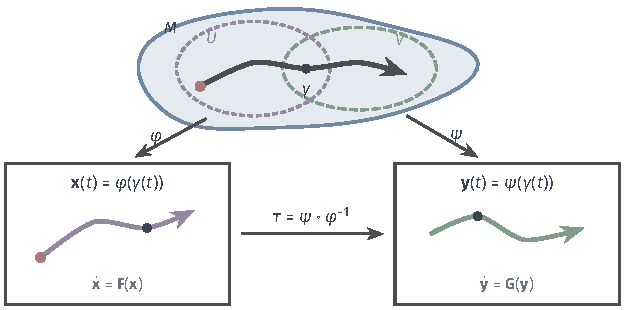
\includegraphics[width=106mm]{figures/06-differential-equations/01-ordinary-differential-equations/tikz/odeex-chart-transfer/figure.pdf}
  \caption{流形上的同一条积分曲线在两张坐标图中的记录。深灰曲线是$M$上的$\gamma$，紫色虚线和绿色虚线围成图的定义域$U,V$，下方是对应的坐标平面，曲线$\bm{x}$与$\bm{y}$分别满足各自的坐标方程。在重叠部分，黑点是同一个状态，转移映射$\tau$把一个方程变成另一个。}
  \label{fig:odeex-chart-transfer}
\end{BookInlineFigure}

\paragraph{局部解的拼接}
现在把第~\ref{sec:odeex-maximal}节的结论逐条搬到流形上。证明的结构不变，只是“盒子”换成坐标图内的盒子，距离的比较只在一张图内进行。

\begin{theorem}[积分曲线]
\label{thm:odeex-manifold}
设$M$是$n$维无边界光滑流形，$X$是其上的光滑向量场。
\begin{enumerate}
 \item 对每个$p\in M$，存在$\varepsilon>0$和积分曲线$\gamma:(-\varepsilon,\varepsilon)\to M$，使$\gamma(0)=p$。
 \item 若两条积分曲线定义在同一区间$I$上，且在某时刻取值相同，则它们在$I$上相同。
 \item 对每个$p\in M$，存在唯一的\term{最大积分曲线}（maximal integral curve）$\gamma_p:I_p\to M$，$\gamma_p(0)=p$，$I_p$是含$0$的开区间，以$p$为起点的积分曲线都是它的限制。
 \item 若$\omega_+=\sup I_p<+\infty$，则对$M$的每个紧子集$C$，存在$t_C\in I_p$，使当$t\in(t_C,\omega_+)$时$\gamma_p(t)\notin C$。
 \item 若$M$紧，则$I_p=\mathbb{R}$对每个$p$成立。
\end{enumerate}
\end{theorem}

\begin{proof}
\emph{结论1。}取含$p$的坐标图，在式~\eqref{eq:odeex-chart-equation}上应用定理~\ref{thm:odeex-picard-lindelof}，得到取值于$\varphi(U)$的解$\bm{x}$，令$\gamma=\varphi^{-1}\circ\bm{x}$。

\emph{结论2。}令$S=\{t\in I:\gamma_1(t)=\gamma_2(t)\}$，它非空。$M$是Hausdorff空间，$M\times M$的对角线闭，映射$t\mapsto(\gamma_1(t),\gamma_2(t))$连续，所以$S$在$I$中闭。

任取$t^\ast\in S$，取含$\gamma_1(t^\ast)$的坐标图$(U,\varphi)$。由连续性，$t^\ast$的某个邻域内两条曲线都留在$U$中，它们的坐标记录都解方程~\eqref{eq:odeex-chart-equation}并在$t^\ast$取相同的值，由定理~\ref{thm:odeex-picard-lindelof}重合。所以$S$在$I$中开，由连通性，$S=I$。

\emph{结论3。}与定理~\ref{thm:odeex-maximal}的证明相同：结论2使所有以$p$为起点的积分曲线相容，它们的并是最大积分曲线；若右端点属于$I_p$，从该点解局部问题就能再延长一段。

\emph{结论4。}先选有限覆盖。对每点$q\in C$取含它的坐标图及其内的一个紧邻域，$C$紧，所以有限个紧邻域$C_1,\ldots,C_r$覆盖$C$，各含于坐标图$(U_i,\varphi_i)$。对紧集$\{0\}\times\varphi_i(C_i)$应用引理~\ref{lem:odeex-uniform-window}，得到时间窗$\delta_i$，令$\delta=\min_i\delta_i$。从$C$的任一点出发的积分曲线至少存在时间$\delta$。

反设存在$t_j\uparrow\omega_+$使$\gamma_p(t_j)\in C$，取$j$使$t_j+\delta>\omega_+$。$X$不显含时间，所以从$\gamma_p(t_j)$出发、再走时间$\delta$的积分曲线平移后接在$\gamma_p$之后，由结论2相容，它越过了$\omega_+$，矛盾。

\emph{结论5。}取$C=M$，$\gamma_p(t)$不可能离开$M$，由结论4，$\sup I_p=+\infty$；对$-X$同样推理，$\inf I_p=-\infty$。
\end{proof}

结论2用到了流形定义中的Hausdorff条件，局部的Picard定理本身用不上它。在双原点直线上取向量场$\partial_x$，从$x=-1$出发的积分曲线到$t=1$时可以到达任一个原点：两条积分曲线在$t<1$时重合，在$t=1$时不同，局部唯一性并不能排除这一点。流形的定义排除了这种空间。满足结论5的向量场称为\term{完备向量场}（complete vector field）。

\paragraph{图内爆炸不是流形上爆炸}
定理~\ref{thm:odeex-escape}用在坐标方程上时，说的是解离开$\varphi(U)$的紧子集，这可能只是走出了这张图。单位圆$S^1$上的匀速转动是最简单的例子。

设$\bm{y}=(\sin\alpha,-\cos\alpha)$，$\alpha=0$是南极，$\alpha=\pi$是北极。令向量场使$\dot\alpha=2$。取从北极出发的球极投影作图：$u=y_1/(1-y_2)$，定义域是$S^1$去掉北极，代入得到$u=\tan(\alpha/2)$。求导，$X$在这张图中的方程是
\[
 \dot u=\frac{1}{2\cos^2(\alpha/2)}\dot\alpha=1+u^2.
\]

从南极出发，$u(0)=0$，解是$u=\tan t$，在$t=\pi/2$时趋于无穷。这与$\dot x=1+x^2$的爆炸是同一个公式，但这里的$u\to\infty$只意味着曲线走向北极，也就是走出了这张图。

换用从南极出发的投影$v=y_1/(1+y_2)$，定义域是$S^1$去掉南极。转移映射是$v=1/u$，所以新图中的方程为
\[
 \dot v=-\frac{\dot u}{u^2}=-\frac{1+u^2}{u^2}=-(1+v^2).
\]
在$t=\pi/4$时，$u=1$，$v=1$。从这里在第二张图中继续解，得到$v=\cot t$，它在$t=\pi/2$时取值$0$，平稳地经过北极。图~\ref{fig:odeex-chart-blowup}显示了这次换图。

\begin{BookInlineFigure}
  \centering
  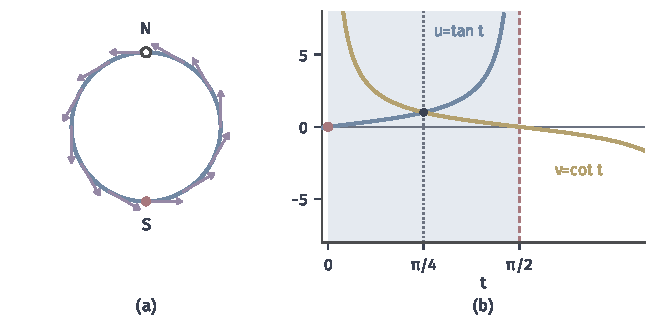
\includegraphics[width=112mm]{figures/06-differential-equations/01-ordinary-differential-equations/matplotlib/odeex-chart-blowup/figure.pdf}
  \caption{图内爆炸不是流形上爆炸。(a)单位圆上的匀速旋转场（紫色箭头），红点是南极$S$，空心点是第一张图未覆盖的北极$N$。(b)蓝线是第一张图的坐标$u=\tan t$，在红色虚线$t=\pi/2$爆炸；黄线是第二张图的坐标$v=\cot t$，在该处取值$0$。黑点是$t=\pi/4$处的换图点，$u=v=1$。}
  \label{fig:odeex-chart-blowup}
\end{BookInlineFigure}

圆是紧流形，由定理~\ref{thm:odeex-manifold}的结论5，积分曲线对所有$t$存在，这里$\alpha=2t$确实如此。

\paragraph{嵌入流形上的切向量场}
流形常常作为$\mathbb{R}^{N}$中的约束集合出现。设$M\subseteq\mathbb{R}^{N}$是嵌入子流形，$W\supseteq M$是开集，$\tilde{\bm{f}}:W\to\mathbb{R}^{N}$光滑，并且在$M$上切于$M$，即$\tilde{\bm{f}}(\bm{p})\in T_{\bm{p}}M$。我们希望知道，从$M$上出发解环境方程$\dot{\bm{y}}=\tilde{\bm{f}}(\bm{y})$，解是否留在$M$上。

唯一性给出的回答很简洁。$\tilde{\bm{f}}$限制在$M$上是$M$的向量场，由定理~\ref{thm:odeex-manifold}有$M$内的积分曲线$\gamma$。把$\gamma$看成$\mathbb{R}^{N}$中的曲线，它就是环境方程的解。环境方程的解是唯一的，所以环境解在$\gamma$存在的时间段内就是$\gamma$，它留在$M$上。约束不需要在算法上另外施加，切向条件加唯一性就够了。

\begin{example}[球面上的旋转场]
\label{ex:odeex-sphere-rotation}
在$\mathbb{R}^{3}$中取$\tilde{\bm{f}}(\bm{y})=(-y_2,y_1,0)$。对$\bm{y}\in S^2$，有$\langle\bm{y},\tilde{\bm{f}}(\bm{y})\rangle=0$，场切于球面。环境方程是线性的，解为绕竖直轴的旋转，保持$\lVert\bm{y}\rVert_2=1$。把$\tilde{\bm{f}}$换成不切的场$(1,0,0)$，解$\bm{y}_0+t(1,0,0)$立即离开球面。
\end{example}

\paragraph{测地线的初值问题}
黎曼流形$(M,g)$上的测地线方程在坐标中写作
\begin{equation}
 \ddot x_k+\sum_{i,j}\Gamma^k_{i,j}(\bm{x})\,\dot x_i\dot x_j=0,\qquad k=1,\ldots,n.
 \label{eq:odeex-geodesic}
\end{equation}
相关的定义可参考\BookChapterRef{chap:riemannian-geometry}{卷四第27章“黎曼几何”}。那里陈述并使用了光滑方程的局部理论，局部存在唯一、最大解和离开紧集三项在这一节得到了证明，光滑依赖由第~\ref{chap:ode-sensitivity}章证明。

它是二阶方程，状态要包括位置和速度。令$\bm{w}=\dot{\bm{x}}$，得到一阶系统
\[
 \dot{\bm{x}}=\bm{w},\qquad\dot w_k=-\sum_{i,j}\Gamma^k_{i,j}(\bm{x})\,w_iw_j.
\]
右端在$\varphi(U)\times\mathbb{R}^{n}$上光滑，定理~\ref{thm:odeex-picard-lindelof}给出局部解。全体$(p,\bm{w})$（$p\in M$，$\bm{w}\in T_pM$）组成的集合称为\term{切丛}（tangent bundle），记为$TM$，它是$2n$维流形，$(\bm{x},\bm{w})$是其坐标。

测地线就是$TM$上一个向量场的积分曲线在$M$上的投影。条件$D\dot\gamma/\mathrm{d}t=0$不依赖坐标，所以不同的图给出的是同一条曲线，定理~\ref{thm:odeex-manifold}的结论都适用：每个初始位置和初始速度决定唯一的最大测地线。

速度的长度沿测地线不变，这给出了$M$紧时的整体结论。设$M$紧，$\lVert\dot\gamma\rVert_g$恒等于初始速度的长度$c$，于是$(\gamma,\dot\gamma)$始终留在集合$\{(p,\bm{w})\in TM:g_p(\bm{w},\bm{w})=c^2\}$中，这个集合是紧的。由结论4，测地线对所有$t$存在。

球面上还可以把测地线写成环境方程，直接看约束是如何保持的。$S^2\subset\mathbb{R}^{3}$的测地线加速度沿法向，方程是
\begin{equation}
 \ddot{\bm{y}}=-\lVert\dot{\bm{y}}\rVert_2^2\,\bm{y}.
 \label{eq:odeex-sphere-geodesic}
\end{equation}
右端是$(\bm{y},\dot{\bm{y}})\in\mathbb{R}^{6}$的光滑函数，在$\mathbb{R}^{3}$中到处都有定义。设初值满足$\lVert\bm{y}(0)\rVert_2=1$和$\langle\bm{y}(0),\dot{\bm{y}}(0)\rangle=0$。

令$c=\lVert\bm{y}\rVert_2^2-1$，$d=\langle\bm{y},\dot{\bm{y}}\rangle$，它们衡量解偏离约束的程度。由式~\eqref{eq:odeex-sphere-geodesic}，
\[
 \dot c=2d,\qquad\dot d=\lVert\dot{\bm{y}}\rVert_2^2+\langle\bm{y},\ddot{\bm{y}}\rangle=-\lVert\dot{\bm{y}}\rVert_2^2\,c.
\]
沿给定的解，$\lVert\dot{\bm{y}}(t)\rVert_2^2$是已知的连续函数，这是关于$(c,d)$的线性系统，初值为零。由唯一性，$(c,d)\equiv\bm{0}$，解永远留在球面上，速度永远切于球面。

取$\bm{p}=(1,0,0)$，$\bm{v}=(0,1,0)$，解是赤道$\bm{y}(t)=(\cos t,\sin t,0)$，此时$\lVert\dot{\bm{y}}\rVert_2^2=1$，$\ddot{\bm{y}}=-\bm{y}$，方程成立。图~\ref{fig:odeex-sphere-constraint}(b)中的蓝线是数值积分得到的$\lVert\bm{y}\rVert_2^2-1$，保持为零。

若初速度不切于球面，例如$\bm{v}=(0.25,1,0)$，则$(c,d)$的初值不为零，$c$随时间偏离零，图中红线的最大值约为$0.39$。约束是否保持，完全取决于初值是否在约束集合上，这正是唯一性的结论。

\begin{BookInlineFigure}
  \centering
  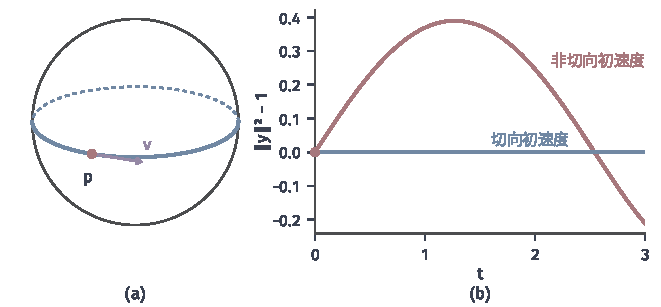
\includegraphics[width=112mm]{figures/06-differential-equations/01-ordinary-differential-equations/matplotlib/odeex-sphere-constraint/figure.pdf}
  \caption{球面测地线的环境方程~\eqref{eq:odeex-sphere-geodesic}。(a)单位球面上过红点$\bm{p}$、初速度为紫色箭头$\bm{v}$的测地线（赤道，背面用虚线）。(b)约束偏差$\lVert\bm{y}\rVert_2^2-1$：蓝线是切向初速度$(0,1,0)$，恒为零；红线是非切向初速度$(0.25,1,0)$，解离开球面。}
  \label{fig:odeex-sphere-constraint}
\end{BookInlineFigure}

平行移动方程
\[
 \dot V_k+\sum_{i,j}\Gamma^k_{i,j}(\bm{x}(t))\,\dot x_iV_j=0
\]
是关于$V$的线性方程，系数沿给定曲线连续。由例~\ref{ex:odeex-linear-global}，它在曲线的整个定义区间上有唯一解，跨图时由唯一性分段接续。测地线方程则是速度的二次方程，局部解未必能延伸到所有时间，这与开单位球上直线走到边界的情形一致，也正是定理~\ref{thm:odeex-escape}所说的状况。
